% -----------------------------------------------
% Template for SMC 2019
% adaed from the template for SMC 2018
% -----------------------------------------------

\documentclass{article}
\usepackage{smc2019}
\usepackage{times}
\usepackage{ifpdf}
\usepackage[english]{babel}
\usepackage{cite}
\usepackage{physics}

%%%%%%%%%%%%%%%%%%%%%%%% Some useful packages %%%%%%%%%%%%%%%%%%%%%%%%%%%%%%%
%%%%%%%%%%%%%%%%%%%%%%%% See related documentation %%%%%%%%%%%%%%%%%%%%%%%%%%
\usepackage{amsmath} % popular packages from Am. Math. Soc. Please use the 
\usepackage{amssymb} % related math environments (split, subequation, cases,
\usepackage{amsfonts}% multline, etc.)
\usepackage{bm}      % Bold Math package, defines the command \bf{}
%\usepackage{paralist}% extended list environments
%%subfig.sty is the modern replacement for subfigure.sty. However, subfig.sty 
%%requires and automatically loads caption.sty which overrides class handling 
%%of captions. To prevent this problem, preload caption.sty with caption=false 
%\usepackage[caption=false]{caption}
%\usepackage[font=footnotesize]{subfig}


%user defined variables
\def\papertitle{Connected Physical Models controlled with the Sensel Morph}
\def\firstauthor{Silvin Willemsen}
\def\secondauthor{Nikolaj Andersson}
\def\thirdauthor{Stefania Serafin}
\def\fourthauthor{Stefan Bilbao}

% adds the automatic
% Saves a lot of output space in PDF... after conversion with the distiller
% Delete if you cannot get PS fonts working on your system.

% pdf-tex settings: detect automatically if run by latex or pdflatex
\newif\ifpdf
\ifx\pdfoutput\relax
\else
   \ifcase\pdfoutput
      \pdffalse
   \else
      \pdftrue
\fi

\ifpdf % compiling with pdflatex
  \usepackage[pdftex,
    pdftitle={\papertitle},
    pdfauthor={\firstauthor, \secondauthor, \thirdauthor},
    bookmarksnumbered, % use section numbers with bookmarks
    pdfstartview=XYZ % start with zoom=100% instead of full screen; 
                     % especially useful if working with a big screen :-)
   ]{hyperref}
  %\pdfcompresslevel=9

  \usepackage[pdftex]{graphicx}
  % declare the path(s) where your graphic files are and their extensions so 
  %you won't have to specify these with every instance of \includegraphics
  \graphicspath{{./figures/}}
  \DeclareGraphicsExtensions{.pdf,.jpeg,.png,.eps}

  \usepackage[figure,table]{hypcap}

\else % compiling with latex
  \usepackage[dvips,
    bookmarksnumbered, % use section numbers with bookmarks
    pdfstartview=XYZ % start with zoom=100% instead of full screen
  ]{hyperref}  % hyperrefs are active in the pdf file after conversion

  \usepackage[dvips]{epsfig,graphicx}
  % declare the path(s) where your graphic files are and their extensions so 
  %you won't have to specify these with every instance of \includegraphics
  \graphicspath{{./figures/}}
  \DeclareGraphicsExtensions{.eps}

  \usepackage[figure,table]{hypcap}
\fi

%setup the hyperref package - make the links black without a surrounding frame
\hypersetup{
    colorlinks,%
    citecolor=black,%
    filecolor=black,%
    linkcolor=black,%
    urlcolor=black
}


% Title.
% ------
\title{\papertitle}

% Authors
% Please note that submissions are NOT anonymous, therefore 
% authors' names have to be VISIBLE in your manuscript. 
%
% Single address
% To use with only one author or several with the same address
% ---------------
\oneauthor
  {Silvin Willemsen, Nikolaj Andersson and Stefania Serafin} { \\ Multisensory Experience Lab, CREATE, Aalborg University Copenhagen \\ %
    {\tt \href{mailto:sil@smcnetwork.org}{\{sil, nsa, sts\}@smcnetwork.org}}}

%Two addresses
%--------------
% \twoauthors
%   {\firstauthor} {Affiliation1 \\ %
%     {\tt \href{mailto:author1@smcnetwork.org}{author1@smcnetwork.org}}}
%   {\secondauthor} {Affiliation2 \\ %
%     {\tt \href{mailto:author2@smcnetwork.org}{author2@smcnetwork.org}}}

% Three addresses
% --------------
%   {\firstauthor} {{} %
%       {}}
%   {\secondauthor} {{Multisensory Experience Lab, CREATE, Aalborg University Copenhagen}
%      {\tt \href{mailto:sil@create.aau.dk}{\{sil, nsa, sts\}@create.aau.dk}}}
%   {\thirdauthor}{
%      {}}
    % {\fourthauthor} { Affiliation4 \\ %
    %  {\tt \href{mailto:author3@smcnetwork.org}{author3@smcnetwork.org}}}


% ***************************************** the document starts here ***************
\begin{document}
%
\capstartfalse
\maketitle
\capstarttrue
%
\begin{abstract}
Lorum Ipsum
\end{abstract}
%

\section{Introduction}\label{sec:introduction}
The behaviour of musical instruments can be well defined by partial differential equations (PDEs).

Finite-difference schemes (FDSs)


The physical models (PMs) used as a case study in this project are the stiff string and the plate.

This paper is structured as follows: Section \ref{sec:PDE} will present the PMs used in our implementation, Section \ref{sec:FDS} will show the how to implement the PMs, Section \ref{sec:connections}

\section{Models}\label{sec:PDE}
In this section, the partial differential equations for the damped stiff string and the plate will be presented. 

% \begin{equation}
%     \pdv[2]{u}{t} = \gamma^2 \pdv[2]{u}{x} -\kappa^2 \pdv[4]{u}{x} - 2\sigma_0\pdv{u}{t} + 2\sigma_1\frac{\partial^3u}{\partial tx^2}
% \end{equation}

\subsection{Stiff string}\label{subsec:stiffStringPDE}
The state $u = u(x,t)$ describes the transverse displacement of the string. The subscript for $u$ denotes a single derivative with respect to time $t$ or space $x$ respectively. The partial differential equation for the damped stiff string is defined as \cite{Bilbao2009:NumericalSoundSynthesis} 
\begin{equation}\label{eq:stiffString}
    u_{tt} = \gamma^2 u_{xx}-\kappa^2u_{xxxx} - 2\sigma_0u_{t} + 2\sigma_1u_{txx},
\end{equation}
where $\gamma$ is wave-speed [m/s], $\kappa$ is stiffness [?] and $\sigma_0 \geq 0$ and $\sigma_1 \geq 0$ are frequency-dependent and frequency-independent damping respectively.

We can add an excitation term to extend Equation \eqref{eq:stiffString} to a bowed string \cite{Bilbao2009:NumericalSoundSynthesis} 
\begin{align}
    \label{eq:bowedString} u_{tt} &= ... - \delta(x-x_\text{B})F_\text{B}\phi(v_\text{rel}) \quad \text{where} \\
    v_\text{rel} &= u_t(x_\text{B}) - v_\text{B},
\end{align}
%the $\delta$ function is only non-zero at the bowing point, effectively locating the bowing interaction.  
where $F_\text{B}$ is the bowing force [N], $v_\text{B}$ is the bowing velocity [m/s], $v_\text{rel}$ is the relative velocity, defined as the difference between the velocity of the string at bowing point $x_\text{B}$ and the bowing velocity $v_\text{B}$ [m/s] and $\phi$ is a friction characteristic, which has been chosen to be \cite{Bilbao2009:NumericalSoundSynthesis}
\begin{equation}
    \phi(v_\text{rel}) = \sqrt{2a}v_\text{rel} \exp(-av_\text{rel}^2+1/2).
\end{equation}

\subsection{Plate}\label{subsec:platePDE}
In the case of a plate, the state $u = u(x,y,t)$ is now defined over two spatial dimensions. The PDE for a damped plate is \cite{Bilbao2009:NumericalSoundSynthesis}

\begin{equation}\label{eq:platePDE}
    u_{tt} = -\kappa^2 \Delta\Delta u - 2 \sigma_0 u_{t} + 2\sigma_1 \Delta u_{t},
\end{equation}
where $\Delta$ represents the 2D Laplacian (also see Equation \eqref{eq:2D}). Just like in the case of the string, an extra term can be added as an input:
\begin{equation}\label{eq:plateExcitation}
    u_{tt} = ... + F_\text{e}E_\text{e},
\end{equation}
where $F_\text{e} = f_\text{e}/ \rho AL$ [m/s$^2$], with bowing force $f_\text{e}$ [N], density $\rho$ [kg/m$^3$], cross-sectional area $A$ [m$^2$] and string length $L$ [m], and $E_\text{e}$ are an excitation function and the excitation area respectively. 

\section{Finite-Difference Schemes}\label{sec:FDS}
To be able to digitally implement the continuous equations mentioned in the previous section, they need to be approximated. The models can be discretised at times $t = nk$, where $n \in \mathbb{W}$ and $k = 1 / f_\text{s}$ is the time-step with sample-rate $f_\text{s}$ and locations $x = lh$, where $l \in [0,N]$ with $N$ being the total number of points and $h$ is the grid-spacing of the model which is calculated differently for each model (see sub-sections below). The discretised variable $u_l^n$ is $u(x,t)$ at the $n$th time step and the $l$th point on the string. In the case of a plate, the second spatial dimension is discretised using $x = lh$ where $l \in [0,N_x]$ with $N_x$ being the total horizontal number of points and $y = mh$ where $m \in [0,N_y]$ with $N_y$ being the total vertical number of points. 
Approximations for the derivatives in the equations found in Section \ref{sec:PDE} are described in the following way: 

When approximating the PDEs shown in Section \ref{sec:PDE}, we use operators 
% \begin{equation}
    \begin{align}
        \label{eq:secondSpacex}\delta_{xx}u_l^n &= \frac{1}{h^2}\big(u_{l+1}^n - 2u_l^n + u_{l-1}^n\big),\\
        % \label{eq:secondSpacey}\delta_{yy}u_l^n &= \frac{1}{h^2}\big(u_{m+1}^n - 2u_m^n + u_{m-1}^n\big),\\
        %  \label{eq:fourthSpace}\delta_xxxx &= \frac{1}{h^4}\big(u_{l+2}^n - 4u_{l+1}^2 + 6 u_{l}^n - 4u_{l-1}^n + u_{l-2}^n\big),\\
        \label{eq:backwardsTime}\delta_{t-} u^n_l &= \frac{1}{k}\big(u_l^{n}-u_l^{n-1}\big),\\
        \label{eq:centerTime}\delta_{t\cdot} u^n_l &= \frac{1}{2k}\big(u_l^{n+1}-u_l^{n-1}\big),\\
        \label{eq:secondTime}\delta_{tt}u_l^n &= \frac{1}{k^2} \big(u_l^{n+1} - 2u_l^n + u_l^{n-1}\big),\\
        % u_{txx} &= \frac{1}{hk^2}\big(u_{l+1}^n - 2u_l^2 + u_{l-1}^n - u_{l+1}^{n-1} + 2u_l^{n-1} - u_{l-1}^{n-1}\big),\\
        % \Delta u &= \frac{1}{h^2}(u_{l, m+1}^{n} + u_{l, m-1}^{n}
        % + u_{l+1, m}^{n} + u_{l-1, m}^{n} - 4u_{l, m}^{n}),\\
         \label{eq:2D}\delta_\Delta u_{l,m}^n &= \frac{1}{h^2}(u_{l,m+1}^n+u_{l,m-1}^n+u_{l+1,m}^n+ \\
         & \qquad \quad u_{l-1,m}^n - 4u_{l,m}^n),
            % \Delta \Delta u &= \frac{1}{h^2}(\Delta u_{l, m+1}^{n} + \Delta u_{l, m-1}^{n},\\
            % & \qquad\quad + \Delta u_{l+1, m}^{n} + \Delta u_{l-1, m}^{n} - 4\Delta u_{l, m}^{n}),\\
        %   \label{eq:biharmonic}   \Delta \Delta u &= u_{xxxx} + 2u_{xxyy} + u_{yyyy}.
    \end{align}
% \end{equation}

\subsection{Stiff String}\label{subsec:stiffStringFDS}
Equation \eqref{eq:bowedString} can be approximated using
\begin{equation}
\begin{aligned}
\delta_{tt} u_l^n =&\gamma^2 \delta_{xx} u_l^n -\kappa^2\delta_{xx}\delta_{xx} u_l^n - 2\sigma_0\delta_{t\cdot} u_l^n  \\
&+ 2\sigma_1\delta_{t-}\delta_{xx}u_l^n - \delta_{x_\text{B}}F_\text{B}\phi(v_\text{rel}),
\end{aligned}
\end{equation}
where $\delta_{x_\text{B}} = \delta(x-x_\text{B})$.
For our implementation, we used clamped boundary conditions, defined as:
\begin{equation}\label{boundary}
    u = u_x = 0 \quad \text{where} \quad l = \{0, N\}.
  \end{equation}
For stability reasons, the grid-spacing needs to abide the following condition
\begin{equation}
    h \geq \sqrt{\frac{\gamma^2 k^2 + 4 \sigma_1 k + \sqrt {(\gamma^2 k^2 + 4 \sigma_1 k)^2 + 16 \kappa^2 k^2}}{2}}.
\end{equation}
The smaller $h$ is, (i.e. the closer $h$ is to this limit), the higher the quality of the implementation. Th number of points $N$ can then be calculated using 
\begin{equation}
    N = h^{-1}.
\end{equation}


\subsection{Plate}
  

Equation \eqref{eq:plateExcitation} can be approximated using
\begin{equation}
    \begin{aligned}
        \delta_{tt}u_{l,m}^n = &-\kappa^2 \delta_\Delta\delta_\Delta u_{l,m}^n - 2\sigma_0\delta_{t\cdot}u_{l,m}^n \\
        &- 2\sigma_1\delta_{t−}\delta_\Delta u_{l,m}^n + F_\text{e}E_\text{e}
    \end{aligned}
\end{equation}

In the case of the plate, we set the number of horizontal and vertical points and calculate grid spacing $h$ from that using 

\begin{equation}
    h = \frac{\sqrt{N_x / N_y}}{N_x}
\end{equation}

\section{Connections}\label{sec:connections}
Adding connections between different PMs, further referred to as elements, adds another term to Equation \eqref{eq:bowedString} or \eqref{eq:plateExcitation}

\begin{align}
    u_{tt} &= ... + F_\alpha E_\alpha, \\
    u_{tt} &= ... + F_\beta E_\beta,
\end{align}
where $F_\alpha$ and $F_\beta$ are the forces of the connection at connection areas $E_\alpha$ and $E_\beta$ respectively. If the a connection area consists of only one point, $E$ reduces to $\delta(x-x_c)$ where $x_c$ is the point of connection. We use the implementation as presented in \cite{Bilbao2009:ModularPercussion} where the connection between two elements is a non-linear spring. The forces it imposes on the elements it connects - denoted by $\alpha$ and $\beta$ - are defined as
\begin{align}
    F_\alpha &= -\omega_0^2\eta - \omega_1^4\eta^3 - 2\sigma_\times\dot\eta,\\
    F_\beta &= -M_{\alpha/\beta}F_\alpha,
\end{align}
where $\omega_0$ and $\omega_1$ are the linear and non-linear spring coefficients respectively, $\sigma_\times$ is the damping factor and $M_{\alpha/\beta}$ is the mass ratio between the two elements. The relative displacement $\eta$ between $\alpha$ and $\beta$ can be calculated as
\begin{equation}
    \eta^n = h_\alpha u_{\alpha, x_\alpha}^n - h_\beta u_{\beta,x_\beta}^n,
\end{equation}
which, in other words, is the difference between the state of element $\alpha$ at connection point $x_\alpha$ and the state of element $\beta$ at connection point $x_\beta$ scaled by their respective grid-spacings $h_\alpha$ and $h_\beta$.

\section{Pitch}
We implemented a damping point in the model that acts as a finger on the (virtual) neck of the instrument controlling pitch. After $u^{n+1}$ is calculated, the following operation is performed at the point of damping:

\begin{equation}
    u_{x_\text{f}}^{n+1} = u_{x_\text{f}}^{n+1}  \sigma_\text{f},
\end{equation}
where $\sigma_\text{f} \in [0,1]$ is the damping coefficient of the finger. 
% put the figure here so it appears on the next page
\begin{figure*}[t]
    \centering
    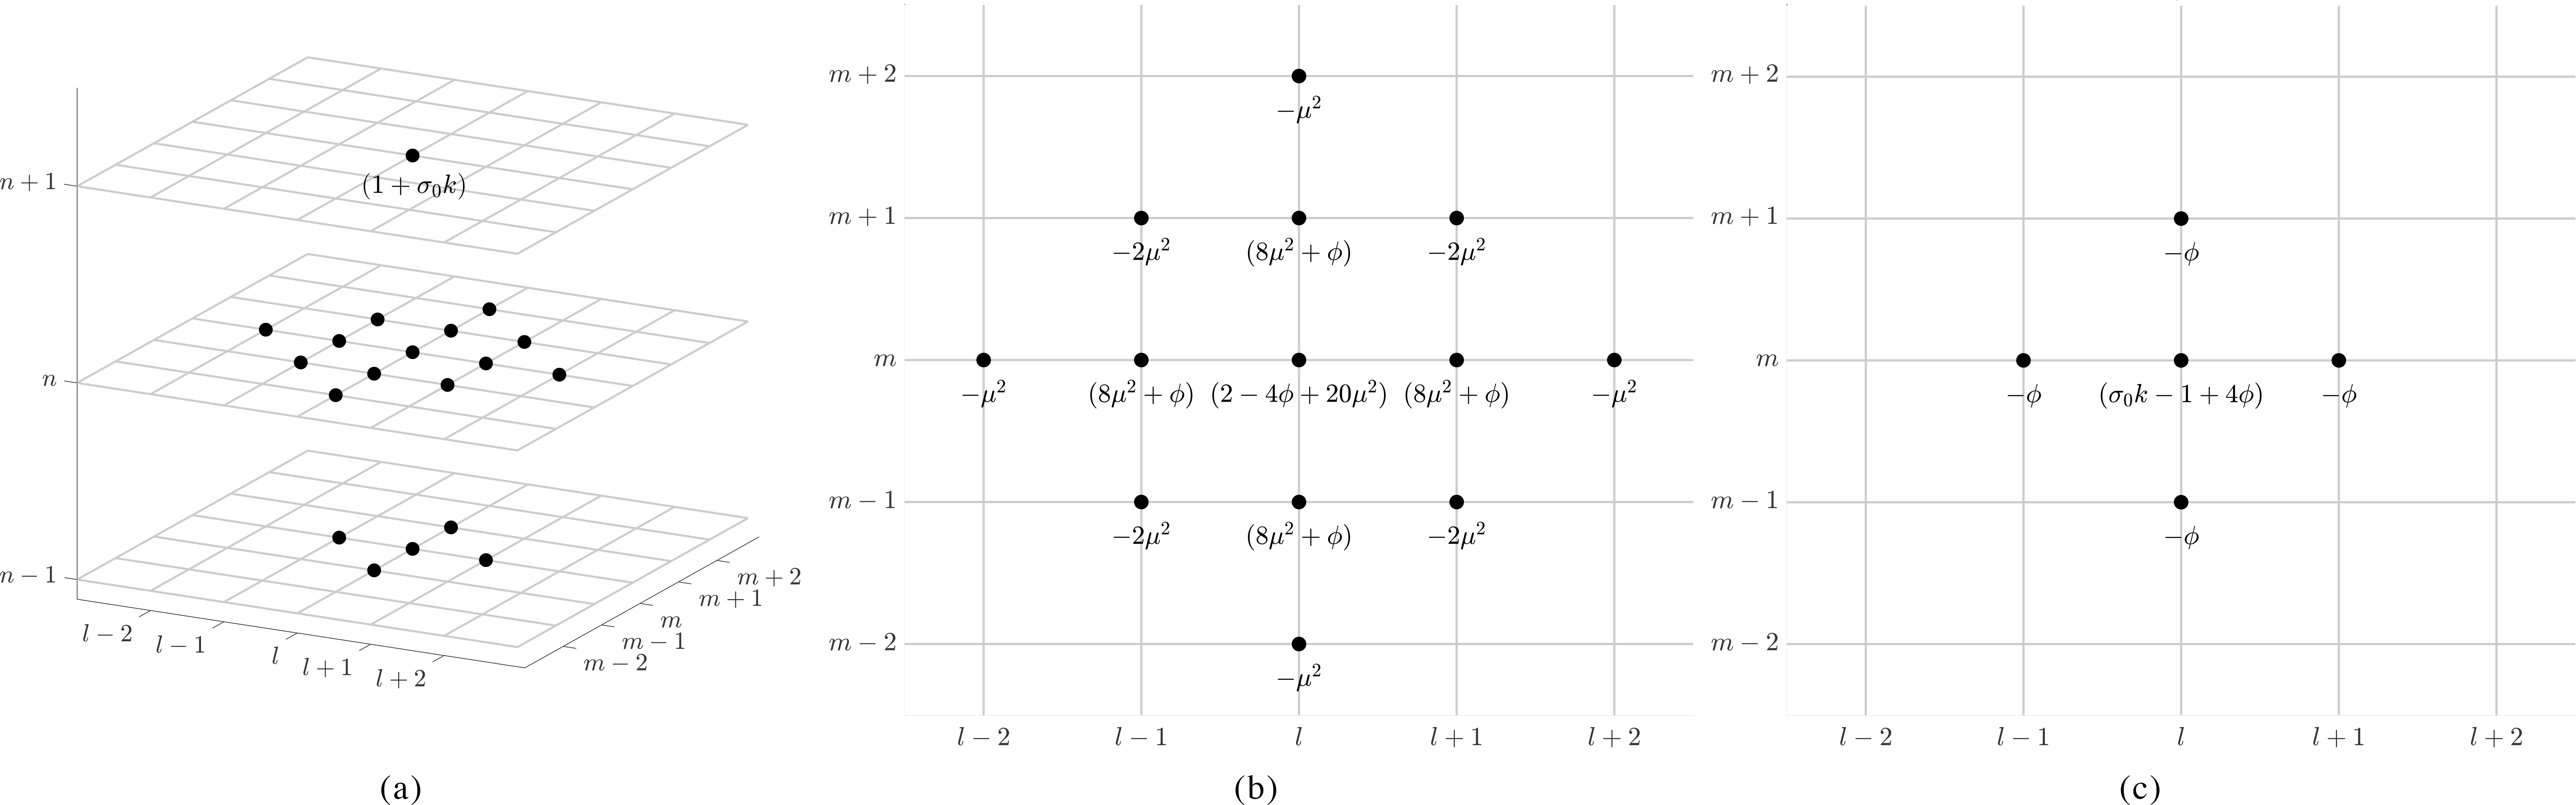
\includegraphics[width=2.1\columnwidth]{FullPlate}
    \caption{A visualisation of Equation \eqref{eq:plateImplementation}. The dots and equations represent the locations $(l,m)$ and what these need to be multiplied with. (a) An overview. (b) The current time-step $n$. (c) The previous time-step $n-1$. \label{fig:example}}
 \end{figure*}
\section{Implementation}
For prototyping \texttt{Matlab} was used. We then used C++ along with the JUCE framework for implementing the objects and connections in real-time.
\subsection{String}
In order to implement the FDSs presented in Section \ref{sec:FDS} they need to be solved for $u^{n+1}$. In the case of the string, we obtain
\begin{equation}
    \begin{aligned}\label{eq:stringImplementatino}
        (1 &+ \sigma_0k)u_l^{n+1} = 2u_l^n - (1 - \sigma_0k) u_l^{n-1} \\
        & +\lambda^2(u_{l+1}^n - 2u_l^n + u_{l-1}^n)\\
        &- \mu^2(u_{l+2}^n - 4u_{l+1}^n + 6u_l^n - 4u_{l-1}^n + u_{l-2}^n) \\
        &+ \frac{2\sigma_1k}{h^2}(u_{l+1}^n - 2u_l^n + u_{l-1}^n\\
        &- u_{l+1}^{n-1} + 2u_l^{n-1} - u_{l-1}^{n-1})\\
        &-k^2\delta_{l_e}F_\text{e},
    \end{aligned}
\end{equation}
where
\begin{equation}\nonumber
\lambda = \frac{\gamma k}{h}\text{,} \quad \mu =  \frac{\kappa k}{h^2} \quad \text{and} \quad \delta_{l_\text{e}} = \delta(x-x_{l_\text{e}}). 
\end{equation}
The wave-speed of the string is proportional to the fundamental frequency of the stiff string according to
\begin{equation}
    \gamma = 2 f_0,
\end{equation}
and the stiffness can be calculated using

\begin{equation}
    \kappa = \frac{\sqrt{B}\gamma}{\pi},
\end{equation}
where $B$ is the inharmonicity coefficient [m$^{-2}$].
The output is retrieved at $l = \text{floor}(0.75N)$ for all strings.

\subsection{Plate}

\begin{equation}
    \begin{aligned}\label{eq:plateImplementation}
        (1& + \sigma_0k)u_{l,m}^{n+1} = (2 - 4\phi + 20\mu^2)u_{l,m}^n\\
    &+ (\sigma_0 k - 1 + 4\phi) u_{l,m}^{n-1}\\
    &-\mu^2 (u_{l,m + 2}^n + u_{l,m - 2}^n + u_{l + 2,m}^n + u_{l - 2,m}^n)\\
    &- 2\mu^2(u_{l + 1,m + 1}^n + u_{l + 1,m - 1}^n + u_{l - 1,m + 1}^n + u_{l - 1,m - 1}^n)\\
    &+ (8\mu^2 + \phi)(u_{l,m + 1}^n + u_{l,m - 1}^n + u_{l + 1,m}^n + u_{l - 1,m}^n)\\
    &- \phi(u_{l,m + 1}^{n-1} + u_{l,m - 1}^{n-1} + u_{l + 1,m}^{n-1} + u_{l - 1,m}^{n-1})\\
    &+ k^2 \delta_{l_\text{e}, m_\text{e}}F_\text{e},
\end{aligned}
\end{equation}
where
\begin{equation}\nonumber
    \mu = \frac{\kappa k}{h^2} \text{,} \quad \phi = \frac{2\sigma_1k}{h^2} \quad \text{and} \quad \delta_{l_\text{e}, m_\text{e}} = \delta(x - x_{l_\text{e}}, y - y_{m_\text{e}}).
\end{equation}

\section{User Interaction}
User-controlled variables:
\begin{itemize}
    \item Bowing position
    \item Bow force
    \item Bow velocity
    \item Connection points
    \item Finger position (pitch)
\end{itemize}

The vertical velocity of the finger is linked to the bow velocity with a maximum of $V_\text{b} = 0.2$ m/s and the finger force is linked to the excitation function with a maximum of $100$m/s$^2$.

\subsection{Sensel Morph}
Something about the sensel morph
\subsubsection{Mapping strategies}
Something about the different prototype mappings, and the "final" mapping 

\section{Discussion}


\section{Conclusion and Future Work}



\begin{acknowledgments}
We would like to thank...
\end{acknowledgments} 

%%%%%%%%%%%%%%%%%%%%%%%%%%%%%%%%%%%%%%%%%%%%%%%%%%%%%%%%%%%%%%%%%%%%%%%%%%%%%
%bibliography here
\bibliography{smc2019bib}

\end{document}
